\section{First approach}

Our first approach to design the system architecture was to develop:

\begin{itemize}
\item A software framework that
abstracted many common concepts found in different social networks (Facebook, Twitter, LinkedIn..)
like User, Post, Reply, Image and so on, to give the developers the possibility to use
(and extend) these abstractions seamlessly between different social networks.

\item A java library to connect, using different interfaces, to the Arduino devices in order
to send the data fetched from the social networks, and also a mechanism to manage Arduino's firmware,
to allow the device to support different configurations.
\end{itemize}

After the second meeting with the customer we decided to revise this plan, as this was not what
our customer really had in mind. Some of the code and documentation we produced earlier could be re-used, but some could not.

See appendix~\ref{app:firstdraftarchi} for more.

\newpage

\section{Revised approach}
The biggest difference in the new design is that API will still provide abstractions
for concepts common to the social network, but it will now focus on estabilishing an interface,
using Android's Intent mechanism, between Social applications and the Android-Arduino applications.

\begin{figure}[h!]
\centering 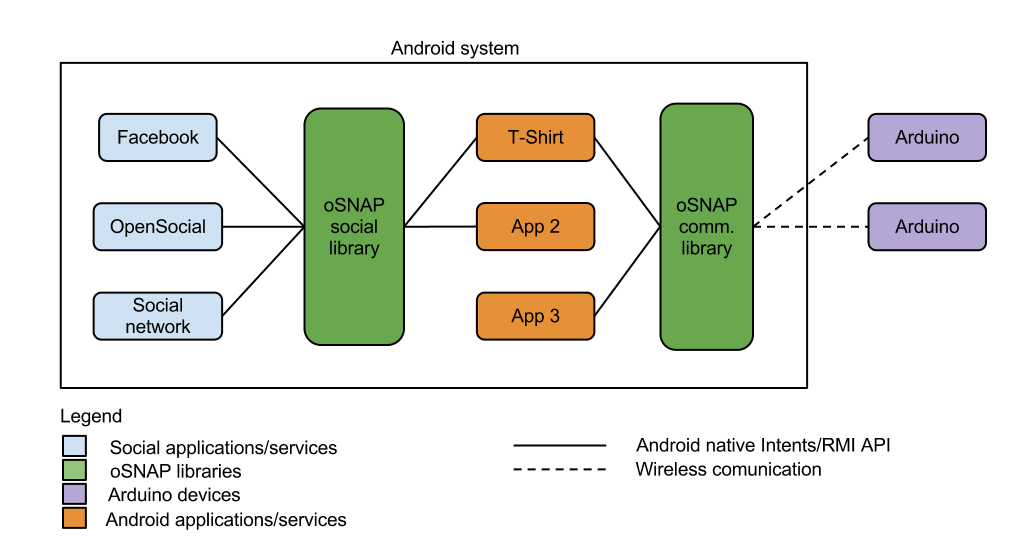
\includegraphics[scale=0.35]{img/architecture-toplevel.png}
\caption{Revised architecture}
\label{fig:architecture-toplevel}
\end{figure}

\newpage

\subsection{First design}
Our first design was based on the scenario where the user would
download the t-shirt and the social applications and then browse for some content
from within the social application and actively send it to the t-shirt application
pressing a 'share' button. This scenario is represented in the following use case.

use case here




\subsection{Second design}


\newpage
\section{Architecture diagram}
The API layer is the social service layer. It uses androids build in broadcast intents to send and
recive data to social services. Included in the social service we have classes that extends Intent
class to indicate if its a social Post, social Group, social Image, social User etc. Multiple apps
can use the API layer to send and retrive this data.

Example:
The API layer is connected with twitter. Twitter retrives a new post and the API layer sends out
a broadcast intent marked as $SOCIAL_POST_IN$. The android OS see who are listeneing to $SOCIAL_POST_IN$ and relay the message to all connected apps. The Developed app now has the post. If the developed app wants to send a post it sends an intent with $SOCIAL_POST_OUT$ that our API can pick up.

The bluetooth protocol in the application is a framework that the developed application includes
to be able to send and recive raw data from the arduino board. It includes handshake and
confirmation commands that is similar to tcp.

The arduino board includes a wrapper around the input/output of the firmware to connect to our protocol.
\begin{figure}[hb!]
\centering 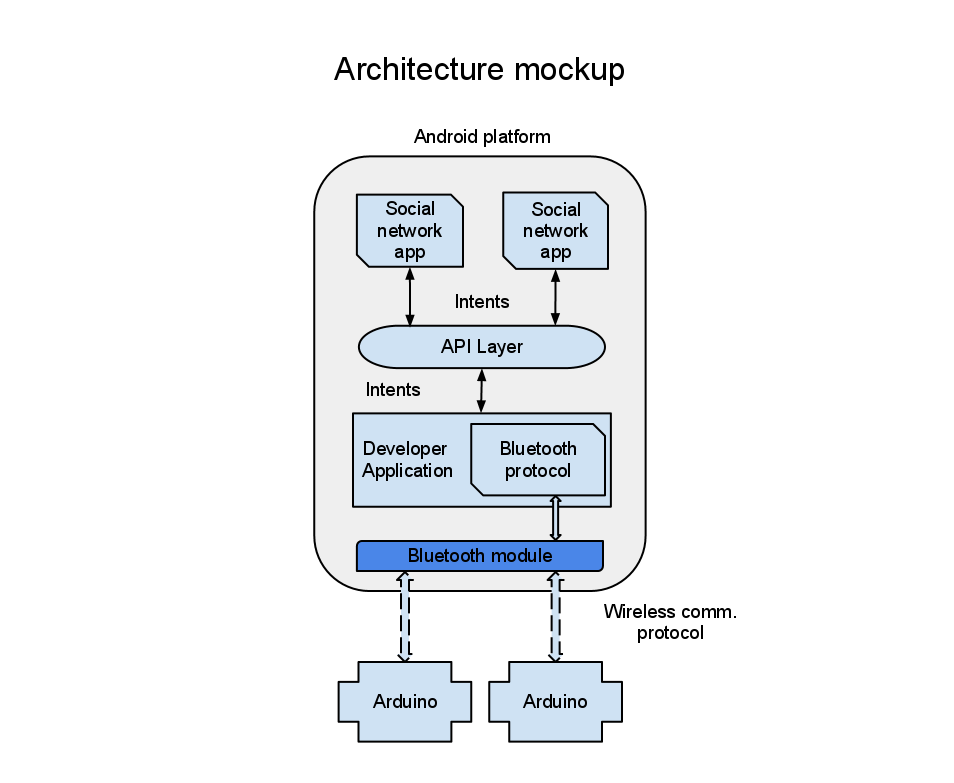
\includegraphics[scale=0.40]{img/architecture-diagram.png}
\caption{System architecture}
\label{fig:architecture-diagram}
\end{figure}

\section{Package Structure}
The system can be divided into smaller sections. This section describes some of the structures
we have divided the system into. The most obvious distinction is between the Java code runs
on the Android platform and the C code which is executed by the Arduino platform.
The Java code is again divided into packaged libraries as described below.

\subsection{Java Code}
\begin{itemize}
\item{no.ntnu.osnap.com}\newline
Communication Library contains every class to establish a connection with a remote device using a general protocol interface. The actual details of the communication such as
Bluetooth, cable, WiFi, stream-based or sockets are hidden away from the user. This is to provide a simple and generic interface to all supported communication methods. The
user can easily add new communication types by extending an abstract class.
\item{no.ntnu.osnap.com.testing}\newline
Test units and sample programs for the ComLib. These are simple test applications that are run on the Android to test if the ComLib is communication correctly using the specified
protocol.
\item{no.ntnu.osnap.social}\newline
Social Library provides an easy to use interface between social networks such as Facebook, Twitter and Myspace and any application or service running on the Android platform.
The SocialLib also provides some general data models such as Person, Group or Post which are concepts that are similar between any social network. 
\item{no.ntnu.osnap.social.testing}  \newline
Test units and sample programs for the SocialLib.
\end{itemize}

\subsection{Arduino C code}
C source code for the Arduino firmware supporting the ComLib protocol.

\newpage
\section{Use cases}
Use Case:
We have two actors we are working with. One is the developer creating the application using our framework. The other one is the end user with the final product. We are not directly working with the end user as an actor, but we still want to make our framework so it is simple for developer to have a product with an easy connection to the arduino board.

Our focus on the actor developer is centered around the software he create. We do not know, and we don't need to know what product he is making. We will work on two parts he can to implement in his software. It will be the setup and transfer protocol to arduino and Intents to send and recive updates from social services.

For the end user, we want the setup to connect his phone to the developer to be as easy as possible. The focus will be on simplified connection to arduino board, and easy connection to social services from application.
\begin{figure}[hb!]
\centering 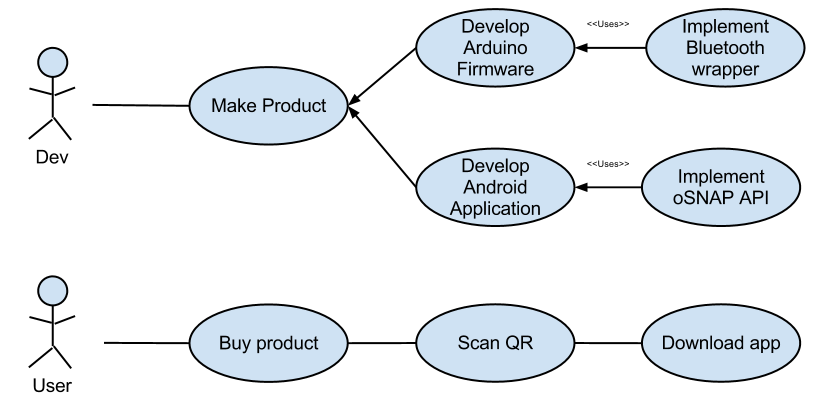
\includegraphics[scale=0.50]{img/use-cases.png}
\caption{Use cases}
\label{fig:architecture-usecases}
\end{figure}

\section{The Protocol}

The protocol is a basic set of rules defined for how devices can communicate to the ardunio. Software needed to be implemented on both sides in addition to these rules to be able to use this protocol. The protocol in itself is created by us, and has seen much editing in terms of which instructions was to be included, and how the communication was to be executed. With the current design the arduino cannot initiate the communication, but is instead a passive device. For all instructions sent by any device to the arduino, the arduino sends a response, if only just to acknowledge that it is finished executing the corresponding tasks. If the instruction is asking for information form the arduino, then the response will contain the corresponding information in the "Content" field. An overview of the current instructions in the protocol can be seen in Table~\ref{tbl:opcodes}.

\begin{table}
	\begin{tabular}{ | c | c | p{1.5cm} | p{1.7cm} | p{6cm} |}
		\hline
		\textbf{Name} & \textbf{OPCODE} & \textbf{Flag} & \textbf{Content} & \textbf{Description} \\ \hline
		Ping & 0x00 & N/A & N/A & Pings the arduino, to check that it's there \\ \hline
		Text & 0x01 & N/A & Text to send & Sends text to the arduino, which then displays it depending on the implementation on the ardunio \\ \hline
		Sensor & 0x02 & Sensor number & N/A & Requests sensor information from the arduino \\ \hline
		Pin pulse & 0x03 & Pin number & N/A & Sends a 500ms pulse on the specified pin \\ \hline
		Pin read & 0x04 & Pin number & N/A & Reads the current digital state of the specified pin on the arduino \\ \hline
		Pin write & 0x05 & Pin number & Pin value (0~or1) & Writes a digital state of a pin on the arduino \\ \hline
		Response & 0xFE & Opcode & Response content & A response to a previous instruction, where the flag is the opcode for which it is the response to \\ \hline
		Reset & 0xFF & N/A & N/A & Resets the arduino \\ \hline
	\end{tabular}
	\caption{Overview of the protocol's instructions}
	\label{tbl:opcodes}
\end{table}

\subsection{Arduino implementation}
On the arduino all code related to our protocol is abstracted into a ComputerSerial library. This library is a very basic state machine which processes single bytes received (see Figure~\ref{fig:arduino_states}). The user of this library can register local methods to be called with RPC when the corresponding instruction is called.

The instructions follow strict rules on how they are constructed (see Table~\ref{tbl:instr_struct} for sizes of the different parts). Each instruction has to start with a "start-byte" which is always 0xFF. The next part is the size, which tells the number of bytes to come for this instruction (including the size byte itself). The rest is defined from which instruction is sent, but it is important to remember that the content cannot be empty, and has to at least contain 1 byte. This byte however, is not necessarily read or used.

\begin{table}
	\begin{tabular}{c|c|c|c|c|c|}
		\cline{2-6}
		& \textbf{Start-byte} & \textbf{Size} & \textbf{Opcode} & \textbf{Flag} & \textbf{Content} \\ \hline
		\multicolumn{1}{|c|}{\textbf{Size}} & 1 & 1 & 1 & 1 & 1-252 \\ \hline
	\end{tabular}
	\caption{The byte-structure of instructions}
	\label{tbl:instr_struct}
\end{table}

\begin{figure}
	\centering
	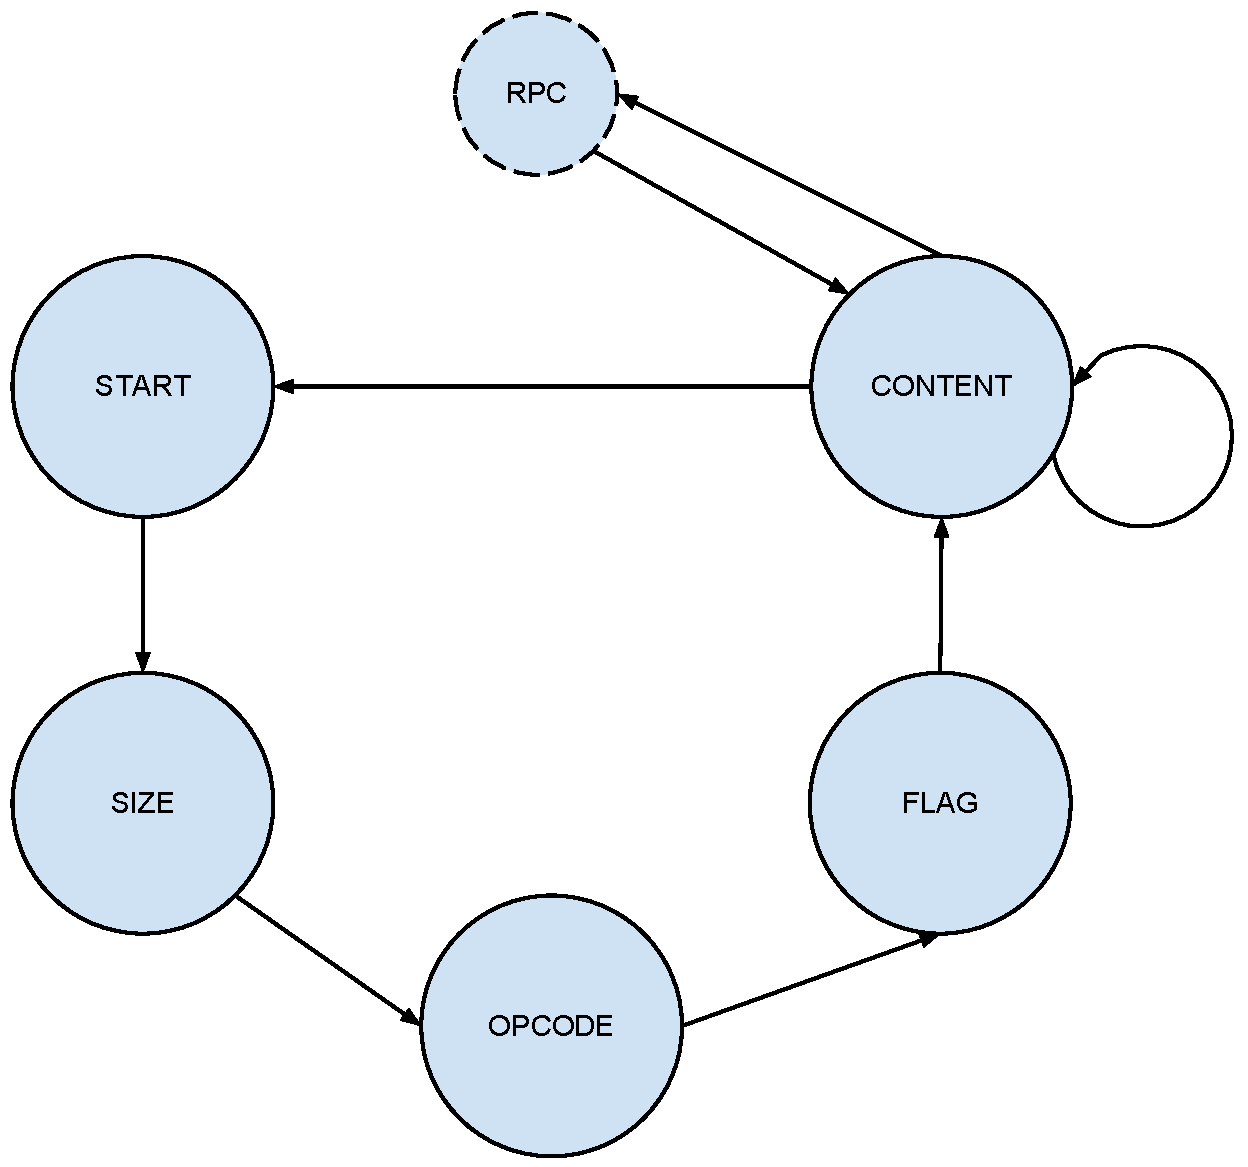
\includegraphics[width=\textwidth, keepaspectratio]{img/arduino_state-machine.pdf}
	\caption{The arduino's state-machine}
	\label{fig:arduino_states}
\end{figure}
